\definecolor{ncp} {RGB}{191,255,191}
\definecolor{car} {RGB}{255,191,255}
\definecolor{bike}{RGB}{255,255,191}
\begin{figure}[H]
  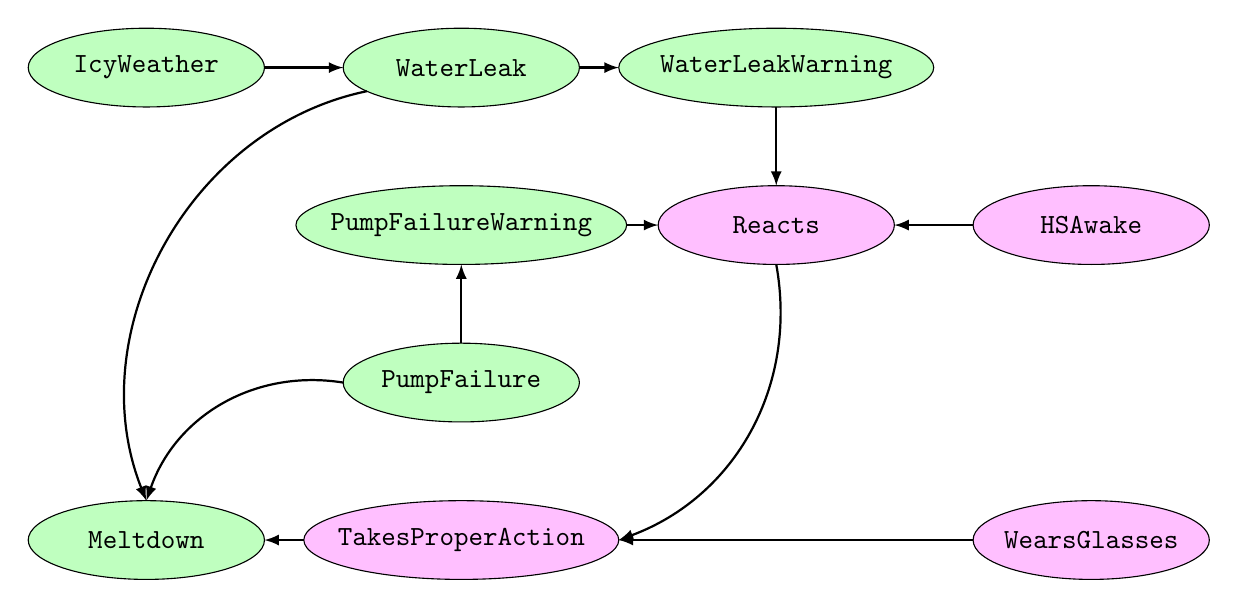
\begin{tikzpicture}

    \draw[fill=ncp] (1,4) ellipse (1.5cm and .5cm) node(a){\texttt{IcyWeather}};
    \draw[fill=ncp] (5,4) ellipse (1.5cm and .5cm) node(b){\texttt{WaterLeak}};
    \draw[fill=ncp] (5,0) ellipse (1.5cm and .5cm) node(c){\texttt{PumpFailure}};
    \draw[fill=ncp] (5,2) ellipse (2.1cm and .5cm) node(d){\texttt{PumpFailureWarning}};
    \draw[fill=ncp] (9,4) ellipse (2cm and .5cm) node(e){\texttt{WaterLeakWarning}};
    \draw[fill=ncp] (1,-2) ellipse (1.5cm and .5cm) node(f){\texttt{Meltdown}};

    \draw[fill=car] (13,2) ellipse (1.5cm and .5cm) node(){\texttt{HSAwake}};
    \draw[fill=car] (9,2) ellipse (1.5cm and .5cm) node(){\texttt{Reacts}};
    \draw[fill=car] (13,-2) ellipse (1.5cm and .5cm) node(){\texttt{WearsGlasses}};
    \draw[fill=car] (5,-2) ellipse (2cm and .5cm) node(){\texttt{TakesProperAction}};

    \draw[arrows={-latex},thick] (2.5,4) to (3.5,4);
    \draw[arrows={-latex},thick] (6.5,4) to (7,4);
%    \draw[arrows={-latex},thick] (5,3.5) to (5,2.5);
    \draw[arrows={-latex},thick] (5,0.5) to (5,1.5);
    \draw[arrows={-latex},thick] (7.1,2) to (7.5,2);
    \draw[arrows={-latex},thick] (9,3.5) to (9,2.5);
    \draw[arrows={-latex},thick] (11.5,2) to (10.5,2);
%    \draw[arrows={-latex},thick] (13,1.5) to (13,-1.5);
    \draw[arrows={-latex},thick] (11.5,-2) to (7,-2);
    \draw[arrows={-latex},thick] (9,1.5) to [bend left=40](7,-2);
    \draw[arrows={-latex},thick] (3,-2) to (2.5,-2);
    \draw[arrows={-latex},thick] (3.8,3.7) to [bend right=50] (1,-1.5);
    \draw[arrows={-latex},thick] (3.5,0) to [bend right=40] (1,-1.5);


  \end{tikzpicture}
  \caption{Bayesian network for meltdown probability with Mr. H.S involved.}
  \label{figHS}
\end{figure}
